\cotefile{57}
\scanpage{22}
simplicity the fibers of $X$ géoém\unsure{t|e}trically normal, and hence $X$ normal !), hence $D$ is linearly equivalent to $0$, what we wanted to prove.

I am convinced however that \uline{Corr} is always separated (with the usual assumptions of properness, flatness, and direct image of the structure sheaf, for both factors,of course). This is easily seen to be true if the \uline{Pic} functor of either factor is representable, by a simple use of dimension theory (namely, we have a morphisme $X\quad\underline{\mathrm{Pic}}_{Y/S}$ whose image has a general fiber of dimension zero, hence the same holds for the special fiber ...). But it is true also, by an immediate adaptation of the same argument, if we suppose only that $\underline{\mathrm{Pic}}_{Y/S}$ is pre-ét-représentable say, i.e. is a quotient of a representable functor $Q$ by an étale equivalence relation (in fact, quasi-finite and flat would do as well), with $Q$ locally of finite type over $S$. Now this assumption is certainly satisfied if $Y$ is \uline{projective} over $S$, as one sees by using the reprsenta\unsure{t|\deleted{t}}tion of $\underline{\mathrm{Pic}}_{Y/S}$ (or rather big open pieces of it) as the quotient of a suitable scheme of immersions of $Y$ into some $P^{r}$, by the action of the projective group operating freely, and taking a quasi-section of the corresponding equivalence relation ... On the other hand, if one does not assume $X$ not $Y$ projective over $S$, one may think of using Chow's lemma; as $S$ is the spectrum of a discrete valuation ring, one does not loose flatness in u\deleted{\unsure{n|u}}sing Chow's lemma, unfortunately one will loose however, I am affraid, the assumption $H^{o}(X_{o},\underline{O}_{X_{o}})\handwritten{\simeq}k(s)$, and I\deleted{a} am affraid that this will make serious technical trouble. Another interesting approach, via topology, is to try to prove that under the usual assumptions on $X$, the ``specialization morphism\deleted{\unsure{e}}'' from the fundamental group of the general geometric fiber to the one of the s\unsure{\deleted{ep}pe|\deleted{pe}ep}cial fiber has an image of finite index - or at least that this is so after
% archive sheet number: 21

\scanpage{23}
making the groups abelian. It seems to me that the latter statement can be proved via the Picard functor, when $X$ is assumed projective over $S$,

I am sending you some notes, including a sketch of the proof of the theorem of representability o\unsure{\deleted{n}f|\deleted{f}n} unramified functors, although I do not think the\deleted{y} latter can be of any use to you, as i have a hard time myself to read them. I think the notes you took when we discussed the matter a few month ago should be much more detailed; anyhow, there are certainly no simplifications in my notes relative to yours, the inverse is more plausible.

Sincerely yours\\
% archive sheet number: 22

\scanpage{73}
July 18, I962\\

My dear Murre,\\

I recently had some thought on finiteness conditions for Picard preschemes, and substantially improved on the results stated in the last section of my last Bourbaki talk. The main result stated there for a simple projective morphism with connected geometric fibers (namely that the pieces $\underline{\mathrm{pic}}^{P}_{X/S}$ are of finite type over $S$) has been extended by Mumford to the case where instead of $f$ simple we assume only $f$ flat with integral geometric fibers,(at least if these are normal). Using his result (the proof of which is quite simple and beautiful) , I could get rid of the normality assumption, and even (as in theorem 4.1. of my talk) restrict to the consideration of the two first non trivial coefficients of the Hilbert polynomials. The key results for the reduction are the following (the proofs being very technical, and rather different for (\unsure{\deleted{a}i|i|1|\deleted{i}a}) and (ii), except that (ii) uses (i) to reduce to the normal case; moreover (ii) uses Mumford's result and the equivalence criteria as developped in my last Seminar):

(i) Let $X$, $Y$ be proper over $S$ neetherian, let $f:X\handwritten{\to}Y$ be a \uline{surjective} $S$ - morphism, assume for simplicity of the statement that the Picard preschemes exist, the\handwritten{n} $f:\underline{\mathrm{Pic}}_{Y/S}\handwritten{\longrightarrow}\underline{\mathrm{Pic}}_{X/S}$ is of finite type (and in fact affine if $S$ is the spectrum of a field), i. e.a subset $M$ of $\underline{\mathrm{Pic}}_{Y/S}$ is quasi-compact iff its image in $\underline{\mathrm{Pic}}_{X/S}$ is.

(ii) The same conclusion holds for a canonical immersion $X\handwritten{\to}Y$, if $Y/S$ is projective with fibers all components of which are of dimension $\handwritten{\geqslant}3$, and if $X$ is the sub-scheme of zeros of a section over $Y$ of an invertible sheaf $\underline{L}$ ample with respect to $S$.

A connected result is that for any $X/S$ proper, and integer $n\handwritten{\ne}0$, the $n$. th power homomorphism in the Picard prescheme is of finite type.

I tell you about this, namely (i), because of the method of proof, involving of course considerations of non flat descent. The fact that I do not have any good effectivity criterion does not hamper, by just recalling what the effectivity of a given descent datum means. Now it turns out that by a slightly more careful analysis of the situation, one can prove the following theorem, of a type very close to the one you have proved recently, and to some you still want to prove as I understand it.

\hfill .../...\par
% archive sheet number: 72

\scanpage{74}
\mspage{2}
\uline{Theorem} Let $S$ be an integral noetherian scheme, $X$ and $\unsure{\mathbb{X}|X}'$ proper over $S$ and $f:X'\quad X$ a surjective $S$-morphism, look at the corresponding homomorphisme for the Picard functors $f^{\bullet}:\text{\uuline{Pic}}_{X/S}\handwritten{\to}\text{\uuline{Pic}}_{X'/S}$. Assume: a) the existence problems A and B defined below for $X/S$ has always a solution (this is certainly true when $X/S$ is projective). b) the morphism $f_{s}:X'_{s}\handwritten{\to}X_{s}$ induced on the generic fiber is a morphism of descent,i.e. $\underline{O}_{X_{s}}\handwritten{\to}f(\underline{O}_{X'_{s}})=h(\underline{O}_{X''_{s}})$ is exact. Then, provided we replace $S$ by a suitable non empty open set, the homomorphism $\unsure{f'|f^{\circ}}$is representable by a quasi-affine morphism, more specifically \unsure{:|;} in the factorisation of $f^{\circ}$via the functor representing suitable descent data, $f^{\circ}=vu$ with $u$ affine and $v$ a monomorphism (as you well know), $v$ is in fact representable by \inserted{\handwritten{finite}} \unsure{divect|divest|divert|direct} sums of immersions.

\uline{Corollary} Without assuming b), but instead in a) allowing $X/S$ to be replaced by suitable other schemes $X_{i}$ finite over $X$, the same conclusion\deleted{s} \deleted{\unsure{are}} holds, namely $f^{\bullet}$is representable by quasi-affine morphisms.

This follows from the theorem, using a suitable factorisation of $f$. For instance, using Chow's lemma and the Main existence theorem in my first talk on Picard schemes, one gets:

\uline{Corollary 2} Assume $X/S$ proper satisfies the condition a') for every $X'$ finite over $X$, there exists a non empty open subset $S_{1}$ of $S$ such that problem A for $X'\quad S_{1}$ has allways solution \deleted{\unsure{of|for|on} problems A and B} (this condition is satisfied if $X/S$ is projective). Then provided we replace $S$ by a suitable $S_{1}$ non empty and open, $\underline{\mathrm{Pic}}_{X/S}$ exists, is separated, its connected components are of finite type over $S$.

\uline{N.B.} The proof does not give any evidence towards the fact that in
\margin{\handwritten{\figure{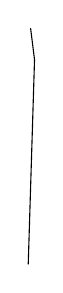
\begin{tikzpicture}\draw (0,0) -- (0.08,2.6) -- (0.03,3.0);\end{tikzpicture}}}}
the theorem, one could replace ``quasi-affine'' by ``affine''. This is true however over a field, bacause a quasi-affine algebraic group is affine ! It would be interesting to have a couterexample,say, over a ring of dimension $1$ such as $k\handwritten{[}t\handwritten{]}$\handwritten{,} $X$ and $X'$ projective and simple over $S$ and $X'\handwritten{\to}X$ birational, or alternatively, $X$ an\handwritten{d}$X'$ projective and normal over $S$, and $f:X'\handwritten{\to}X$ finite. A counterexample in the latter case would of course provide a counterrexample to the effectivity problem for a finite morphism raised in my first talk on descent ....

``Problem A'' is the following: given $X/S$ and Module $F$ on $X$, to represent the functor on the category of $S$-preschemes taking any $S'/S$ into a one-element or into the empty set, occording as to whether $F'$ on $X'/S'$ is flat with respect to $S'$ or not, where $X'=X\mathbin{x}_{S}S'$, $F'=F\mathbin{x}_{S}S'$.

\hfill .../...\par
% archive sheet number: 73

\scanpage{75}
\mspage{3}
Given $X/S$, we say that ``Problem A for $X/S$ has always a solution '' if for every coherent $F'$ on some $X'/S'$, the previous functor on $(\handwritten{\mathrm{Sch}})/S'$ is representable by a $S'$-scheme of finite type. The main step in my proof of existence of Hilbert schemes shows that this condition is satisfied when $X/S$ is projective; In the proof, essential use is made of the Hilbert polynomial, in fact we get a solution as a disjoint sum of subschemes of $S$ corresponding to various Hilbert polynomials. Still I would expect that the functor is representable as soon as $X/S$ is proper. In view of the application we have in mind here, it would be sufficient (for any \unsure{intugral|integral} $S$) to find in $S$ a non empty open set $S_{1}$ such Problem A has always a solution for $X_{1}=X\mathbin{x}_{S}S_{1}$ over $S_{1}$. \unsure{To|Tb} prove this weeker existence result, it is well possible that a reduction to the projective case is possible, using Chow's lemma and some induction on the relative dimension perhaps. I also would expect that a proof wil be easier when working over a complete noetherian local ring, hence the case of a general noetherian local ring by flat descent. And it is well possible that, putting together two such partial results, a proof of the existence in general could be obtained. (I met with such difficulties allready time ago in a very analoguous non projective existence problem, which beside I did not solve so far !). This problem A has been met also by Hartshorne (A Harvard Student), but I doubt he will work seriously on it. Thus I now wrote you in the hope you may be interested to have a try on this problem. \unsure{As a|Asa} general fact, our knowledge of non projective existence theorems is exceedingly poor, and I hope this will change eventually.

Sincerely yours.\\

A. GROTHENDIECK\\
% archive sheet number: 74

\scanpage{76}
\handwritten{July 18, 1962}\\

My dear Murre,\\

I recently had some thought on finiteness conditions for Picard preschemes, and substantially improved on the results stated in the last section of my last Bourbaki talk. The main result stated there for a simple \deleted{\unsure{morphism (namely that|morphism(with $X$ prjt|morphism(with $Y$ prjt}}\inserted{projective morphism} with connected geometric fibers (namely that the pieces $\underline{\mathrm{Pic}}^{P}_{X/S}$ are of finite type over $S$) has been extended by Mumford to the case where \deleted{the fibers} instead of $f$ simple we assume only $f$ flat with integral geometric fibers,\inserted{(at least if these are normal).} Using his result (the proof of which is quite simple and beautiful), I could get rid of the normality assumption, and even (as in theorem 4.1. of my talk) restrict to the consideration of the two first non trivial coefficients of the Hilbert polynomials. The key results for the reduction are the following (the proofsbeing very technical, and rather different for (i) and (ii), except that (ii) uses (i)\deleted{and Mumford's} \unsure{\deleted{h}t|\deleted{t}h}o reduce to the normal case; moreover (ii) uses Mumford's result and the equivalence criteria as developped in my last Seminar):

(i) Let $X,Y$ be proper over $S$ noetherian, let $f:X\handwritten{\to}Y$ be a \inserted{\uline{surjective}} $S$-morphis\handwritten{m,} \deleted{m,} assume for simplicity of the statement that the Picard preschemes exist, the $f^{\bullet}:\underline{\mathrm{Pic}}_{Y/S}\handwritten{\to}\underline{\mathrm{Pic}}_{X/S}$ is of finite type (and in fact affine if $S$ is the spectrum of a field), i.e. a subset $M$ of $\underline{\mathrm{Pic}}_{Y/S}$ is quasi-compact iff its image in $\underline{\mathrm{Pic}}_{X/S}$ is .

(ii) The same conclusion holds for a canonical immersion $X\handwritten{\to}Y$, if $Y/S$ is projective with fibers all components of which are of dimension $\handwritten{\geqslant}3$, and if $X$ is the sub-scheme of zeros of a section over $Y$ of an invertible sheaf $\underline{L}$ ample with respect to $S$.

A connected result is that for any $X/S$ proper, and integer $n\handwritten{\ne}0$,
% archive sheet number: 75

\scanpage{77}
the $n$.th power homomorphism in the Picard prescheme is of finite type.

I tell you about this, namely (i), because of the method of proof, involving of course considerations of non flat descent. The fact that I do not have any good effectivity criterion does not hamper, by just recalling what the effectivity of a given descent datum means. \deleted{By a} Now it turns out that by a slightly more careful analysis of the situation, one can prove the following theorem, of a type very close to the one you have proved recently, and \inserted{\handwritten{to}} some you still want to prove as I understand it\deleted{\unsure{:}}.

\uline{Theorem} Let $S$ be an integral noetherian scheme, $X$ and $X\handwritten{'}$ proper over $S$ and $f:X\handwritten{'\to}X$ a surjective $S$-morphism, look at the corresponding homomorphisme for the Picard functors $f^{\bullet}:\underline{\underline{\unsure{\mathbb{P}|P}\mathrm{ic}}}_{X/S}\handwritten{\to}\text{\uuline{Pic}}_{X\handwritten{'}/S}$ . Assume: a) the existence problem\deleted{s} A \deleted{and B} defined below for $X/S$ ha\deleted{v}\handwritten{s}\deleted{e} always a solution (this is certainly true when $X/S$ is projective). b) the morphism\deleted{\unsure{e}} $f_{s}:X\handwritten{'}_{s}\handwritten{\to}X_{s}$ induced on the generic fiber is a morphism of descent, i.e. $\underline{O}_{X_{s}}\handwritten{\to}\deleted{\unsure{g}}\handwritten{f_{*}}(\underline{O}_{X\handwritten{'}_{s}})\handwritten{\unsure{\rightrightarrows|\substack{\longrightarrow\\[-0.7ex]\rule{1.4em}{0.4pt}}}}h_{\handwritten{\unsure{*|\uparrow}}}(\underline{O}_{X''_{s}})$ is exact. Then, \uline{provided we replace $S$ by a suitable non empty open set},\margin{\handwritten{\unsure{$\epsilon$|e|c|$\in$} not\\ needed ?}} the homomorphism\deleted{\unsure{e}} $f^{\bullet}$ is representable by \deleted{a} quasi-affine morphism\deleted{s}, more specifically \deleted{the} in the factorisation of $f^{\circ}$via the functor representing suitable descent data, $f^{\bullet}=vu$ with $u$\unsure{.} affine \deleted{\unsure{as you know,both|as you know, both}} and $v$ a monomorphism (as you well know), $v$ is in fact representable by \inserted{\handwritten{finite direct sums of}} immersions.

\uline{Corollary \handwritten{\unsure{1|!}}} Without assuming b), but instead in a) allowing $X/S$ to be replaced by suitable other schemes $X_{i}$ finite over $\unsure{\mathbb{X}|X}$, the same conclusion holds, namely $\unsure{f^{\circ}|f^{\bullet}}$ is representable by \deleted{\unsure{finite|finit}} quasi-affine morphisms.

This follows from the theorem, using a suitable factorisation of
% archive sheet number: 76

\scanpage{78}
$f$. For instance, using Chow's lemma and the Main existence theorem in my first talk on Picard schemes, one gets:

\uline{Corollary} 2\quad Assume $X/S$ proper satisfies the condition\unsure{;|:}\deleted{\unsure{a') for every}} \deleted{\unsure{any $X'$}\illegible{2} for} a') for every $X'$ finite over $X$, there \unsure{exist|exists} a non empty open subset $S_1$ of $S$ such that \inserted{\handwritten{problem A for}} $X'\handwritten{\mid}S_1$ has allways solution \deleted{for problems A and B} (this condition is satisfied if $X/S$ is projective). Then \deleted{there exists} provided we replace $S$ by a suitable $S_1$ non empty and open, $\underline{\mathrm{Pic}}_{X/S}$ exists, is separated, its connected components are of finite type over $S$.

N.B. The proof does not give any evidence towards the fact that in the theorem, one could replace ``quasi-affine'' by ``affine'' . This is true however over a \unsure{fiéèd|fièèd|field}, because a quasi-affine algebraic group is affine ! It would be interesting to have a couterexample, say,over a \deleted{valuation} ring of dimension $1$ such as $k\handwritten{[}t\handwritten{]}$ , $X$ and $X'$
\figure{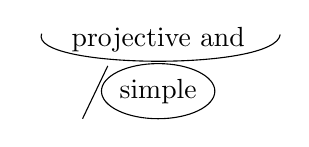
\begin{tikzpicture}
  \node[inner sep=0pt] (addition) at (0,0.65) {\inserted{projective and}};
  \node[inner sep=0pt] (simple) at (0,0) {simple};
  \handwritten{
    \draw (-1.48,0.73) .. controls (-1.65,0.28) and (1.50,0.25) .. (1.55,0.72);
    \draw (simple.center) ellipse (0.72cm and 0.35cm);
    \draw (-0.96,-0.35) -- (-0.64,0.32);
  }
\end{tikzpicture}}
\reversemarginpar
\margin{\handwritten{\figure{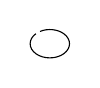
\begin{tikzpicture}\draw (-0.18,0.13) arc[start angle=135,end angle=480,x radius=0.25cm,y radius=0.18cm];\end{tikzpicture}}impossible if\\$X$ smooth !}}
\normalmarginpar
\noindent over $S$ and $X'\handwritten{\to}X$ birational,\unsure{orx|or\deleted{r}|orr} alternatively, \deleted{\unsure{if $X'$ finite}} $X$ and $X'$ projective and normal over $S$, and $f:X'\handwritten{\to}X$ finite. A counterexample in the latter case would of course provide a couterexample to the effectivity
\figure{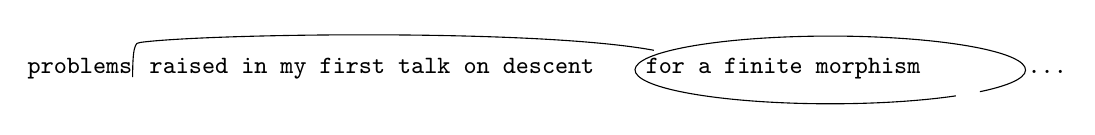
\begin{tikzpicture}[every node/.style={font=\small\ttfamily,inner sep=0pt,anchor=base west}]
  \node (problem) at (0,0) {problem\deleted{\unsure{s}}};
  % The circled phrase is attached after problem by the drawn return line.
  % It remains at its typed physical position on the right in this reproduction.
  \node (morphism) at (7.85,0) {\inserted{for a finite morphism}};
  \node (raised) at (1.55,0) {raised in my first talk on descent};
  \node at (12.70,0) {\dots};
  \handwritten{
    \draw (12.10,-0.236) arc[start angle=320,end angle=670,x radius=2.48cm,y radius=0.43cm];
    \draw (7.96,0.29) .. controls (6.45,0.57) and (2.25,0.50) .. (1.44,0.39)
      .. controls (1.37,0.40) and (1.34,0.32) .. (1.34,-0.05);
  }
\end{tikzpicture}}

``Problem A'' is the following: given $X/S$ and \deleted{any} Module $F$ on $X$, to represent the functor on the category of $S$-preschemes taking any $S'/S$ into \deleted{the empty or} into a one-element \inserted{or into the empty} set; according as to wheter $F'$ on $X'/S'$ is flat with respect to $S'$\inserted{\handwritten{or not}}, where $X'=X\mathbin{x}_S S'$, $F'=F\unsure{2|x|\otimes}_S S'$ . Given $X/S$, we say that ``Problem A \inserted{\handwritten{for $X/S$}} has always a solution'' if for every coherent $F\handwritten{'}$ on \deleted{$X$}\inserted{\handwritten{some $X'/S'$}}, the previous functor \inserted{\handwritten{on $(\mathrm{Sch})/S'$}} is representable by a \inserted{$S\handwritten{'}$\handwritten{-}}scheme of finite type. The main step in my proof of existence of Hilbert schemes shows that this condition is satisfied when $X/S$ is projective,
% archive sheet number: 77

\scanpage{79}
In the proof, essential use is made of the Hilbert polynomial, in fact we get a solution as a disjoint sum of subschemes of $S$ corresponding to various Hilbert polynomials. Still I would expect that the \deleted{\unsure{solution}} functor is representable as soon as $X/S$ is proper. In view of the application we have in mind here, it would be sufficient (for an\unsure{\deleted{y}|y} integral $S$) to findin $S$ a non empty \deleted{\unsure{set}} open set $S_{\unsure{1|i}}$ such Problem A has always a solution for $X_1=X\mathbin{x}_S S_1$ over $S_1$ . To prove this weeker existence result, it is well possible that a reduction to the projective case is possible, using Chow's lemma and some induction on the relative \unsure{dimension} perhaps. I also would expect that a proof will be easier when working over a complete noetherian local ring, hence the case of a
% The source fragment is drawn once to retain the interlinear word and the hand correction strokes. The baseline word local remains live.
\begin{minipage}[c]{4.7cm}
\figure{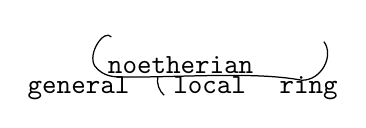
\begin{tikzpicture}[x=1cm,y=1cm]
  \node[anchor=base west,inner sep=0pt,font=\ttfamily] at (0,0) {general};
  \node[anchor=base west,inner sep=0pt,font=\ttfamily] at (1.85,0) {local};
  \node[anchor=base west,inner sep=0pt,font=\ttfamily] at (3.20,0) {ring};
  \node[anchor=base west,inner sep=0pt,font=\ttfamily] at (1.02,0.25) {\inserted{noetherian}};
  \handwritten{
  \draw[line width=0.45pt] (1.07,0.72)
    .. controls (0.98,0.83) and (0.76,0.51) .. (0.86,0.35)
    .. controls (0.97,0.21) and (1.11,0.21) .. (1.25,0.21)
    .. controls (2.04,0.21) and (2.91,0.28) .. (3.49,0.17)
    .. controls (3.74,0.17) and (3.90,0.48) .. (3.77,0.66);
  \draw[line width=0.45pt] (1.66,0.22)
    .. controls (1.64,0.13) and (1.68,0.03) .. (1.74,-0.02);
  }
\end{tikzpicture}}
\end{minipage}
by flat descent. And it is well possible that, putting together two such partial results, a proof of the existence in general could be obtained. (I met with such difficulties allready time ago in a very \unsure{analognous|analoguous} non projective existence problem, which beside I did not solve so far !). This problem A has been met also by Hartshorne (a Harvard student), but I doubt he will work seriously on it. Thus \deleted{to}\handwritten{\unsure{J|I}} now wrote you in the hope you may be interested to have a try on this problem. As a general fact , our knowledge of non projective existence theorems is exceedingly poor, and I hope this will change eventually.

\noindent\hspace*{1cm}Sincerely yours\hfill\handwritten{A Grothendieck}\par
% archive sheet number: 78

\cotefile{63}
\scanpage{3}
\begin{center}\uline{Contents}\end{center}

\noindent 1. Generalized Weierstrass form \qquad p~1.

\noindent 2. Change of coördinates \qquad p~2.

\noindent 3. \unsure{'}Minimal \unsure{Weierstrass|weierstrass} equations over a valuation ring \qquad p~3.

\noindent 4. The canonical filtration on the group of $v$-adic points \qquad p~4.

\noindent 5. Application. The relation between $L_v(1)$ and $\int_{E_v}|\omega_v|$ in case $k$ is finite \qquad p~6.

\noindent 6. The Neron minimum model \qquad p~\unsure{7.|?}

\noindent 7, Algorithm for analysing singular fibers \quad (first five cases) \qquad p~8.

\noindent 8. Algorithm continued \quad (last five cases) \qquad p~10.

% archive sheet number: 2
